\documentclass[a4paper]{scrreprt}
\usepackage[utf8]{inputenc}
\usepackage[T1]{fontenc}
%--------------------------------------------------
\usepackage[english]{babel}		% English language 
\usepackage{lmodern}					% font looks better on screen
\usepackage{microtype}				% even better
\usepackage{fullpage}					% more space on the page
\usepackage{natbib}

% Math symbols and stuff
%--------------------------------------------------
\usepackage{amsmath}					% all the fancy math stuff
% \usepackage{amssymb}					% more math symbols
% \usepackage{wasysym}					% even MORE math symbols
% \usepackage{upgreek}					% upright Greek letters

% Enhanced formatting
%--------------------------------------------------
\usepackage{color}						% enable color
% \usepackage{colortbl}					% colored tables
\usepackage{graphicx}					% fancy graphics
% \usepackage{wrapfig}					% wrap figures
% \usepackage{tabularx}					% better tables
\usepackage{enumerate}				% customize numbered lists
% \usepackage{tocloft}					% fancy table of content
% \usepackage{caption}					% extended captioning, e.g. without numbers
% \usepackage{fancyhdr}					% fancy header customisation
% \usepackage[parfill]{parskip} % vspace instead of indentation
% \usepackage{geometry}					% customize page size, margins etc
\usepackage{listings}         % code listings
\usepackage{paralist}						% inline lists

% Extra stuff, glossary, index etc
%--------------------------------------------------
% \usepackage{glossaries}				% glossaries
% \usepackage{makeidx}					% index
% \usepackage{showidx}					% print index items for debugging
\usepackage{url}							% URL handling
\usepackage{hyperref} 				% should be loaded last
% \usepackage{syntonly}					% check for syntax only; much faster
% \syntaxonly										% comment if output is desired
% \renewcommand{\cftsecleader}{\cftdotfill{\cftdotsep}}	% dots in TOC

% Stuff that doesn't fit in any category
% \usepackage{lastpage}					% provides total number of pages, use with:
%																% \pageref{LastPage}
\usepackage{xspace}
\usepackage{blindtext}
%-------------------------------------------------- 

% setup the listings package
\lstset{%
	language=perl,
	basicstyle=,          % the size of the fonts that are used for the code
	numbers=left,                      % where to put the line-numbers
	numberstyle=\tiny,         % the size of the fonts that are used for the line-numbers
	%stepnumber=2,                      % the step between two line-numbers. If it is 1 each line will be numbered
	numbersep=5pt,                     % how far the line numbers are from the code
	backgroundcolor=\color{lightgrey}, % choose the background color. You must add \usepackage{color}
	showspaces=false,                  % show spaces adding particular underscores
	showstringspaces=false,            % underline spaces within strings
	showtabs=false,                    % show tabs 
	frame=none,                        % can be: none, leftline, topline, bottomline, lines, single, shadowbox 
	%frameround=tttt,                   % rounded corners; t=round, f=corner
	tabsize=2,                         % sets default tabsize to 2 spaces
	captionpos=t,                      % caption position (t|b)
	breaklines=true,                   % automatic line breaking
	breakatwhitespace=false,           % automatic breaks should not happen at whitespace
	%escapeinside={\%}{)}              % if you want to add a comment within your code
}

% setup hyperlinks
\hypersetup{%
	bookmarks=true,
	pdftitle={ORTHOGRAPH},
	pdfauthor={Malte Petersen},
	pdfcreator={pdflatex},
	pdfsubject={orthology prediction},
	pdfkeywords={orthology} {prediction} {est} {transcriptome} {phylogeny}
}

% new colors and commands
\definecolor{lightgrey}{rgb}{0.9,0.9,0.9}
\newcommand{\file}[1]{{\lstinline{#1}}}
\newcommand{\code}[1]{{\texttt{#1}}}
\newcommand{\hamstr}{HaMStR\xspace}
\newcommand{\pname}{ORTHOGRAPH\xspace}
\newcommand{\species}[1]{\textit{#1}}


\linespread{1.3}

\title{Fast and efficient mapping of transcript sequences to ortholog groups}
\subtitle{\pname: ORTHOlogy prediction using a Graph-based, Reciprocal Approach with Profile Hidden Markov models}
\author{Malte Petersen}

\begin{document}
%\frontmatter
\maketitle
\tableofcontents

%\mainmatter
\chapter{Journal}
\section{August - November 2011}
\subsection*{2011-08-15 Treffen mit Oliver/Karen}

\begin{figure}[h]
	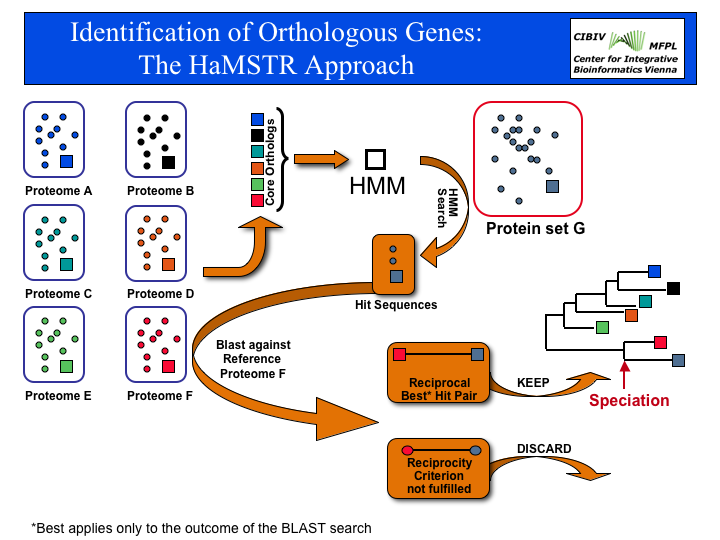
\includegraphics[width=\textwidth]{img/hamstr-schema.png}
	\caption{\cite{Ebersberger2009}}
\end{figure}

Tasks:

\begin{itemize}
	\item read paper
	\item install HaMStR, test
	\item read \& understand the source:
		\begin{itemize}
			\item what is happening when
			\item at what point does it use genewise?
		\end{itemize}
	\item look up:
		\begin{itemize}
		\item genewise/exonerate (alignment NA $\rightarrow$ AA)
			\item PAL2NAL
			\item ESTwiseDB
			\item BLASTx (what does it do)
		\end{itemize}
\end{itemize}

Vortrag beim Montagskolloquium über DA (desinteressiertes, ahnungsloses
Publikum)

\begin{itemize}
	\item Warum?
\end{itemize}

\subsection*{2011-08-16}

Installed HaMStR v8 with all dependencies:

\begin{table}[h]
	\begin{tabular}{l l l}
		\textbf{Package} & \textbf{Version} & \textbf{Source}\\
		\hline
		HMMer    & 3.0	 & http://www.deep-phylogeny.org/hamstr/download/ \\
		ClustalW & 2.1   & ftp://ftp.ebi.ac.uk/pub/software/unix/wise2/ \\
		Genewise & 2.2.0 & http://hmmer.janelia.org/software \\
	\end{tabular}
\end{table}

All programs were installed in PATH. With Genewise, a modification was
necessary in \file{src/HMMer2/sqio.c}: renamed getline() to genewise\_getline()
since getline() is already defined in \file{stdio.h} (standard C library).

All test runs according to the README files were successful.

Read the HaMStR paper (\cite{Ebersberger2009}).

Tried to get an insurance for the lab key, so far unsuccessful.

\subsection*{2011-08-17}

Picked up playground data and annotations from Karen.

\subsection*{2011-08-18 What does HaMStR do?}

Genewise: At the very end, \emph{after} the re-BLAST. Translates ESTs to
revcomp, only if at least one hit was obtained.

\subsection*{2011-08-23 Karen}

\begin{itemize}
	\item ``transitive closure'' $\rightarrow$ lookup \url{deep-phylogeny.org}
	\item InParanoid: Orthology by pairwise assignment
	\item OrthoMCL: Orthology by pairwise $\rightarrow$ groups of orthologs. Read
		presentations.
	\item parallelize: spawn daughter processes according to \#CPU?
\end{itemize}

\subsection*{2011-08-24 Oliver}

``deep search'': blast instead of hmmsearch (weniger sensitiv)

``very deep search'': hmm hits mit estwisedb (übersetzen und suchen in 1) gegen
core-orthologs

Warum nur orthologe Gene durchsuchen? $\rightarrow$ auch nicht orthologe,
vielleicht passen sie besser.

EST-Set schrittweise verkleinern\dots

Benchmarks mit absichtlich verschlechterten Sequenzen, z.B. einen von den
Core-Orthologen zufällig verändern.

\begin{table}
	\begin{tabular}{l l}
	\textbf{program} & \textbf{compares} \\
	\hline
	genewise   & single protein vs single DNA seq \\
	genewisedb & protein database vs DNA database \\
	estwise    & single protein vs single EST/cDNA seq \\
	estwisedb  & protein database vs EST/cDNA database
	\end{tabular}
\end{table}

valid command line:
\begin{verbatim}
../hamstrsearch_local-hmmer3.v8.pl
-sequence_file=cleaned/Adelphocoris_lineolatus_contig.fa
-fasta_file=ortholog_set_insecta_hmmer3-1/insecta_hmmer3-1.fa -taxon=apime
-refspec=dappu_1391 -blast_path=ortholog_set_insecta_hmmer3-1/blast_dir -est
\end{verbatim}

\section{September 2011}
\subsection*{2011-09-02}

Karen nach Erklärung fragen:
\renewcommand{\labelenumi}{\alph{enumi})}
\begin{enumerate}
	\item Frameshifts + deren Korrektur
	\item Introns + interne Stopcodons: Wie erkennen und sinnvoll entfernen?
\end{enumerate}

\includegraphics[width=0.5\textwidth]{img/hamstr-cmdline-files.pdf}
\begin{table}[h]
\begin{tabular}{l l l}
	\textcircled{A} & cleaned/Adelphocoris\_lineolatus\_contig.fa & $\leftarrow$ EST file (fasta)\\
	\textcircled{B} & ortholog\_set\_insecta\_hmmer3-1/insecta\_hmmer3-1.fa & $\leftarrow$ Core ortholog set (fasta)\\
	\textcircled{C} & dappu\_1391 & $\leftarrow$ reference taxon, from the core set \\
	 \textcircled{D} & ortholog\_set\_insecta\_hmmer3-1/blast\_dir & $\leftarrow$ BLAST database for the re-BLAST
\end{tabular}
\end{table}

\subsection*{2011-09-05 $\rightarrow$ 11 Started writing FORAGE}

\textbf{F}ind \textbf{O}rthologs using \textbf{R}eciprocity \textbf{A}mong
\textbf{G}enes and \textbf{E}STs 

\begin{description}
\item[Forage, v.:] Durchsuchen, (nach Nahrung) suchen etc.
\end{description}

There are BioPerl modules for 
\begin{enumerate}
	\item translation to all 6 reading frames
	\item using HMMer
	\item using BLAST
	\item reading \& writing files
\end{enumerate}
(but Oliver and Bernhard think I should stay away from them)

\subsection*{Intranet}

\fbox{\lstinline{boutEST\&Protein!2011}}

\begin{tabular}[h]{l l}
	\url{svzfmksql03} & $\rightarrow$ Server \\
	\url{131.220.75.253} & ~\\
	\url{lpd://131.220.75.250/przfmk010} & PPD: Apple 12/640ps\\
	\url{przfmk010} & 2. Etage\\
	\url{przfmk09} & 1. Etage\\
	\url{domzfmk} & Domain\\
	\url{131.220.228.166} & Cluster (pwd zfmk)\\
	\url{131.220.228.163} & alter Cluster\\
\end{tabular}

VPN? $\rightarrow$ Christoph fragen

\begin{lstlisting}
smbclient -W DOMZFMK -U <username> //SVZFMKSQL03/Molekular-Labor
\end{lstlisting}

\verb|mount.cifs| in \file{fstab}:
\begin{lstlisting}
//svzfmksql03/molekularlabor/ /mnt/zfmknet cifs noauto,users,credentials=/path/to/credsfile 0 0
\end{lstlisting}

\subsection*{2011-09-14}

Fiddled around with BioPerl, tried to reproduce Hamstr

hmmfound nothing in Andrena\_vaga $\rightarrow$ can this be true? Double-check!

\vspace{1em}
\begin{minipage}{0.4\textwidth}
	\begin{itemize}
		\item Substitute Unix tools w/ builtin Perl functions, e.g. grep/sed
		\item Debugging
		\item InParanoid source?
		\item CC license
		\item ``Forage''
		\item Computer?
	\end{itemize}
\end{minipage}
\hfill
\begin{minipage}{0.5\textwidth}
\textbf{PRIORITÄTEN}
\renewcommand{\labelenumi}{\arabic{enumi}.}
	\begin{enumerate}
		\item Korrigierte Nucleotide-Seq zu den Amino-Alignments die Hamstr
		ausspuckt $\rightarrow$ genewise-output speichern und parsen $\rightarrow$ pal2nal,
		sonst exonerate $\rightarrow$ Gerrit fragen! Prob?
		\item Orthologen-Set erstellen
	\end{enumerate}
\url{(arthropods.)eugenes.org}
\end{minipage}

\subsection*{2011-09-15}

be paranoid about BioPerl

\subsection*{2011-09-27 after I got this lab journal back\dots}

how the data structure could look like in Forage:

\begin{verbatim}
             {EST ID}
                 |
                 v
{seq, matched_by_hmm, hmm_score}
\end{verbatim}

how the data structure looks like in Hamstr:
\begin{verbatim}
            {taxon}
               |
               v
{prot=>hmm-hit seq, ids=>hmmhits, refseq=>refspec-seq, refspec=>refspec}
\end{verbatim}

\subsection*{2011-09-28}

\begin{lstlisting}
	$gw->{gw}	# ref to array
	print join("\n", @$gw->{gw})	# "not an ARRAY reference" error
	my $out = $gw->{gw};
	print join("\n", @$out); # works -> WTF?
\end{lstlisting}

Solution: dereferencing done correctly: 
\begin{lstlisting}
	print join("\n", @{$gw->{gw}}
\end{lstlisting}

\begin{itemize}
	\item ursprüngliche, korrigierte Nuc-Sequenz fehlt im Hamstr-output
	\item steht in genewise-output?
	\item sonst exonerate
	\item testen was genewise ausspuckt, wenn seq.\ künstlich verändert
	$\rightarrow$ frameshift, zus.\ A etc
\end{itemize}

\subsection*{2011-09-30 genewise splittet bei frameshifts}

\subsection*{2011-09-X cluster access}

\url{mptersen@131.220.228.166} pwd \url{zfmk}

List of installed software: \url{131.220.75.250}

Queueing system:

\begin{table}[h]
	\begin{tabular}{l l l}
	\verb|qsub| & <bash script> & (multiple opts for the script\dots RTFM)\\
	\verb|qstat| & show running stuff & (\verb|-f| full output)\\
	\verb|qdel| & delete jobs & ~ \\
	\verb|qhost| & show running stuff & (\verb|-j| by all users)\\
	\verb|mpirun| & for MPI & $\rightarrow$ only where it makes sense, read docs
	first!
	\end{tabular}
\end{table}

important: no relative paths in scripts

\section{October 2011}
\subsection*{2011-10-05}
\begin{verbatim}
	genewise -cdna -trans -sum -pep
\end{verbatim}
\verb|-gff| mögl.? $\rightarrow$ cdna zum pep-Alignment speichern, pal2nal

\verb|s/genewise/exonerate/ ?|

\subsection*{2011-10-18 been working on substitution of genewise by exonerate}
genewise is 
\begin{inparaenum}
	\item slower, 
	\item less able and 
	\item does not output cDNA for its translation.
\end{inparaenum}

exonerate is
\begin{inparaenum}
	\item fast,
	\item more precise (does not cut off as much as genewise if there are
	frameshifts), and 
	\item does output cDNA instead of the translation.
\end{inparaenum}

The cDNA sequences are desired.

Done so far:
\begin{itemize}
	\item reproduced genewise output in exonerate (sp, pep, sp.tr)
	\item modified run\_genewise\_hamstr.pm to run exonerate instead of genewise
	(now called exonerate.pm)
\end{itemize}

\begin{description}
\item[discoveries:] the exonerate package brings along a number of fasta-file
modification tools, including \emph{fastatranslate}, which can \emph{100\%
replace} the BioPerl translate\_6frames and is \textasciitilde 10x faster
(written in C)
\item[problems:] exonerate has no means of outputting the \# of indels - this is
used by Hamstr to determine how to concatenate the seq fragments after
translation
\item[$\rightarrow$] if there are indels, they are tr'ed to lower case, if not,
represented as 'N'
\end{description}

\section{December 2011}
\subsection*{Thu Dec  1 00:01:30 CET 2011}

Finally fixed and manicured the cdna bug in Hamstr. It now works as expected,
including corresponding cdna output. I still want to optimize the terminal
messages.

Jeanne wrote a script that creates a Hamstr-compatible core ortholog set from a
bunch of OGS FASTA files. Apart from a few bugs which may already be fixed, it
works very well already. It runs fastatranslate, muscle/mafft and hmmbuild and
takes a couple of hours. I used a newly generated ortholog set with Hymenoptera
(mostly ants) and let Hamstr chew on Andrena vaga with it, and it appears to
work very well, spits out beautifully matching sequences. 

Tanja has been working on a summarizer script that packs the Hamstr output into
human-readable form. In particular, it compiles the AA sequences of all the
hamstred taxa along with the core orthologs in one FASTA file, aligns it and
cuts out the core ortholog seqs again so that we are left with the aligned query
taxon seqs. Very nice and useful. She has been doing a lot of careful work, and
has now been provided with real-life output to test and fine-tune her script
with.

I have to start preparing the presentation for the MoKo on Dec 19th. Oliver has
given me a couple of valuable tips for structure, content and design. Will
probably do the thing in \LaTeX\ again, I am beginning to really like the beamer
package. Along with the textpos package, positioning graphics and stuff anywhere
I want is no longer a hassle. And it just looks so beautiful\ldots

\subsection*{Fri Dec  2 18:40:54 CET 2011}

Didn't do anything in Hamstr the last two days. Rather, was of assistance to
Jeanne and Tanja and had a couple of discussions with Karen/Oliver/Bernhard.
Tanja accidentally uncovered a problem when summarizing the Hamstr output: When
a sequence contains stop codons (TAA, TAG, TGA), they will be cut out/replaced
with gaps by MUSCLE or MAFFT. Therefore, and since we want them conserved, Tanja
will replace them with 'x' before the alignment step and replace them back once
the alignment is complete. MAFFT allows to preserve case, MUSCLE does not.
Tanjas Program will only use MAFFT-LINSI in the future.

I was a little surprised that nobody seemed to have given the stop codons any
thought so far. Do they carry phylogenetic information? How do they influence the
tree inference? How do they mutate, if they do at all? I'll have to look this
up. I wrote a small script to check the sequence lengths of amino acid and
nucleotide output, but they always match. Hamstr itself does nothing to the stop
codons.

Jeanne is getting bored; she needs a challenge. Even adding the nucleotide to
the newly generated core ortholog set isn't going to take her more than a day, I
think. I wonder if I could think about something that would really make her
ponder\ldots Something like the prime numbers that she would think about more
than a day. I don't know. Maybe I'll introduce her to \url{projecteuler.com}
next week.

Yesterday, Alex did his Momento talk about the new cluster. It went quite well,
but took too long, I think. 

\subsection*{Sun Dec 11 14:37:13 CET 2011}

Jeanne's and Tanja's lab module ended on Friday. They both finished the
programs they worked on, and although Karen and I didn't get a chance to test
them, they appear work fine. Well, I hope so, because none of us is going to
find the time to bug-fix or really work on them. They did leave a good
impression, though, and maybe one (or both) of them will write their master's
thesis here, as well. 

I started working on FORAGE again, too. Exchanged Path::Class for File::Spec and
re-wrote the hmmsearch output parser so that pre-existing result files are not
skipped, but their content is made available. Now everything is ready to get out
the hits and do the reciprocal search.

Tomorrow I'm flying to Vienna because they made me :) No, I'm excited what to
expect there, I've never been to a real scientific meeting before. Karen, Caro,
Bernhard and I are going to visit another work group there that is also part of
the 1KITE project (\url{1kite.org}). I'm also going to give the ten-minute talk
about HaMStR and my thesis there, which I'm also going to give the Monday after
in the MoKo. I've been polishing it for days and I think it's in a semantically
sensible structure now. I hope everybody thinks the same when I give it for real.

\subsection*{Wed Dec 14 22:27:45 CET 2011}

I just got back from Vienna and am waiting for the train home. These last few
days have been extraordinarily great for me, which is why I will allow some more
intimate thoughts in this journal tonight. 

We visited the work groups of Nicola Szucsich and Daniela Bartels at the
University of Vienna from Monday to today. We departed Cologne at 0650 (in the
morning - gah!) and landed in Vienna some one and a half hour later and took the
trains straight to the university and met that work group. These people are so
nice and friendly\ldots It has really been a pleasant surprise meeting them,
although I am normally very wary of meeting new people. Anyway, we had coffee
and then Karen spoke for over four hours about ESTs and what we do with them.
Not about Hamstr, that has been saved for Tuesday. Nicola and Dani had a lot of
questions, especially about the sequence assemblers and MARE. What puzzled them
most was the way the four competing tree topologies were not only generated, but
also scored and compared. How can there be more than one topology for a given
dataset in a ML analysis? I don't even remember\ldots that part was in the late
afternoon, and I was having a low and very nearly fell asleep during that
discussion.

In the evening, we rode to Nicola and Dani's. They live together, have a young
child and are apparently very much in love with each other. Very nice to watch,
especially seeing a university professor on his knees, in a dirty sweater, and
trying to talk his daughter into pushing a triangular brick into a triangular
hole. If anything, it only made him more human. Hannah, their daughter, was very
cool. Well, we had dinner and sat until midnight.

The next day, Bernhard arrived, and I gave my talk, which I have been polishing
thoroughly. 

\subsection*{Wed Dec 28 18:34:30 CET 2011}

Didn't finish reporting about Vienna -- nevermind. 

I got back to FORAGE the last few days before Christmas. The Forage::Item module
is now fully object-oriented, the class abstraction layer is complete. No more
direct access to the object data like in Hamstr :P 

In the new year, I can't wait to get to the reciprocal search part. I did some
performance test and found out the following:

\begin{description}
	\item[open, while readline] seems to be the fastest way of finding
	a certain string in a file. 
	\item[open, read into array, grep] is slower, and requires more memory.
	\item[Tie::File] is awfully slow.
	\item[system calls to grep] are also very fast, but probably have more
	overhead because of the system call, and add to platform independence issues.
\end{description}

I am going to use the \lstinline{while readline} approach for getting the
sequences from the EST file for the reciprocal search. How can I use hmmsearch
for that? From the HMMer manual, page 32:

\begin{quote}
HMMER uses an ad hoc sequence weighting algorithm to downweight closely related
sequences and up-weight distantly related ones. This has the effect of making
models less biased by uneven phylogenetic representation. For example, two
identical sequences would typically each receive half the weight that one
sequence would. 
\end{quote}

So apparently the more diverse the ortholog set, the more sensitive the HMMs.
Maybe that is why the ortholog sets from Ebersberger contain not only insecta,
but also worms, diptera, butterflies and ants. These things have to be tested,
but can I do that in my thesis? 


\section{January 2012}
\subsection*{Thu Jan  5 17:21:04 CET 2012}
A typical header that comes out of fastatranslate looks like this:
\begin{verbatim}
>N_30845_l_412_cov_76_830093 [revcomp]:[translate(3)]
\end{verbatim}
\begin{quote}
Dear Mr Slater,

I'm using your excellent exonerate package in an orthology prediction pipeline
that I am writing for my diploma thesis at the ZFMK, Bonn, Germany. I was also
been very happy that you provide binary tools for handling fasta files -
especially fastatranslate is finding central use in my pipeline. Thanks for
making my life that much easier!

Today, it came to my mind that instead of looping through a fasta file in Perl
or using external tools like grep, I could use fastaindex and fastafetch to get
individual sequences. However, fastaindex refuses to index a file that was
previously translated using fastatranslate because of non-unique sequence
identifiers. I think that these occur because fastatranslate uses whitespace to
separate the original fasta header from the "[translate(n)]" information, and
fastaindex appears to not recognise these as individual headers.  
\end{quote}

I dug into the exonerate source and replaced the space with an underscore in
\file{src/sequence/sequence.c}:

\begin{lstlisting}[language=c,caption=src/sequence/sequence.c]
void Sequence_print_fasta(Sequence *s, FILE *fp, gboolean show_info){
    fprintf(fp, ">%s", s->id?s->id:"[unknown]");
    if(s->def)
        fprintf(fp, "_%s", s->def);	//mp s/_/ /
    if(show_info){
        if(s->strand != Sequence_Strand_UNKNOWN)
            fprintf(fp, "_[%s]", (s->strand == Sequence_Strand_FORWARD)	//mp s/_/ /
                               ?"forward":"revcomp");
        if(s->alphabet->type != Alphabet_Type_UNKNOWN)
            fprintf(fp, "_[%s]",	//mp s/_/ /
                    Alphabet_Type_get_name(s->alphabet->type));
        if(s->len)
            fprintf(fp, "_[length %d]", s->len);	//mp s/_/ /
        }
    fprintf(fp, "\n");
    Sequence_print_fasta_block(s, fp);
    return;
    }
\end{lstlisting}

But I wonder if that's the right thing to do. Maybe at other places this messes
things up, for example in the hmmsearch output, where the translation info is
conveniently moved to the description part. I also found the part where the
sequence file is parsed by the fasta* tools, but I am hesitant to change it,
because this might seriously mess up other parts in exonerate (these tools all
use the same codebase). I could use Perl to find the sequences, it might even be
sufficiently fast, but I'd like to be as efficient as possible. I am going to
find a solution to this. 

\subsection*{Mon Jan 16 14:05:58 CET 2012}

Started integrating MySQL into Forage. The things that are now possible are
amazing\ldots Oliver and I have agreed on using MySQL entirely wherever
possible. It is not only faster by orders of magnitude when searching for a
specific sequence, but also does it allow centralizing the results and enable
highly flexible output formats for future applications. I learned everything I
needed in two days and am still discovering new things.

\subsubsection*{JOIN}

\lstset{language=SQL}
\begin{lstlisting}
SELECT ests.hdr, ests.seq, hmmsearch.hmmhit, hmmsearch.hmm FROM ests JOIN hmmsearch ON ests.hdr = hmmsearch.hmmhit;
\end{lstlisting}
Output: Rows from ests and hmmsearch where \lstinline{est.hdr == hmmsearch.hmmhit}

\begin{lstlisting}
SELECT ests.hdr, ests.seq, hmmsearch.hmmhit, hmmsearch.hmm FROM ests INNER JOIN ests ON ests.hdr = hmmsearch.hmmhit;
\end{lstlisting}
Output: Rows from ests and hmmsearch where \lstinline{est.hdr == hmmsearch.hmmhit}. 
If they do not match, they will not be output. INNER JOIN joins when all
criteria are fulfilled.


\section{February 2012}
\subsection*{Fri Feb 24 18:13:31 CET 2012}

The database structure was redesigned to something far less redundant and more
useful. It is not fully integrated into Forage, though. I'm still busy with the
helper script to set up the database structure in the first place. Two weeks ago
I finally passed the last exam in cytology! 

1KITE is making progress fast, too. At the moment we are busy compiling our
ortholog set for usage in Hamstr. There has been an agreement to use OrthoDB
(\url{http://cegg.unige.ch/orthodb}), and last week Karen and I hand-picked the
matching genomes from all the taxa we are using from all over the web. The
version and everything has to match exactly the proteome version that was used
in OrthoDB, otherwise we will not be able to get corresponding nucleotide output
from Hamstr. 

\subsection*{Sun Feb 26 20:58:46 CET 2012}

Read two papers about HMMer3 (\cite{Eddy2009}) and the position-specific scoring
matrices that \lstinline{hmmbuild} uses for generation of the profiles
(\cite{Henikoff1994}) because we want to dig deeper into how HMMer calculates
its profile hidden Markov models and how more or less diverse sequences impact
the overall sensitivity of a model. As far as I understood, more diverse
positions get a bonus weight, while more common positions get a penalty. Since
the whole model is position-specific, the total sequence weight is of limited
importance. Hidden Markov models are also position-specific and predict the
occurence of a nucleotide or amino acid in one position based on the nucleotide
or amino acid in the previous position(s) using a fairly complex probability
calculation that involves hidden Markov models (HMMs). I should really
understand those.

I don't have those papers with me right now, so I'll summarize them next time.

Oliver helped in getting those OGS that we need to create our ortholog sets.
Maybe next week we can start compiling everything together and then use Tanja's
script with corresponding nucleotide output for the first time.

\section{March 2012}
\subsection*{Mon Mar 19 11:45:32 CET 2012}

During the 2$^nd$ half of Feb, I tutored the LSI course one last time. When I
returned, I spent a lot of time on the HMM test and its report. 

\section{April 2012}
\subsection*{Fri Apr 13 16:38:22 CEST 2012}

The proteome files for Forage (or more specifically, coreload) must have a very
restrictive header format: Only the protein ID is accepted, otherwise coreload
gets confused. Coreload is going to check for this.

\section{August 2012}
\subsection*{Fri Aug 31 17:58:27 CEST 2012}

My thesis should be structured like this:

\begin{enumerate}
	\item Orthology prediction:
	\begin{itemize}
		\item why is it important?
		\item what are the different approaches?
		\item why is the graph-based approach better than the tree-based one?
	\end{itemize}

\item \hamstr:
	\begin{itemize}
		\item hidden Markov models:
			\begin{itemize}
				\item what are HMMs?
				\item why do they represent homology better than a similarity alignment?
			\end{itemize}
		\item what did \hamstr right?
		\item what did \hamstr wrong/what could be improved in this approach?
	\end{itemize}

\item \pname:
	\begin{itemize}
		\item why did I rewrite instead of extending \hamstr?
		\item why did I use a database?
		\item why did I try parallelization?
	\end{itemize}

\item Results:
	\begin{itemize}
		\item same/better hit rate as \hamstr?
		\item test different ortholog sets?
		\item test simulated data?
	\end{itemize}
\end{enumerate}


\chapter{Orthology prediction}
In morphological phylogenies, so called homologous characters are used to
reconstruct ancestral trees. The term homolog was introduced in 1843
(\cite{owen1848}) and was used to describe ``the same organ in different animals
under different every variety of form and function''. Similarly, analogs were
defined as ``part or organ in one animal which has the same function as another
part or organ in a different animal''. In the famous \emph{Origin of Species}
(\cite{darwin1859}), the term homology is never used, but in a review
(\cite{owen1860}), homology is referred to as evidence of evolution.

A morphological character is the phenotypic reflection of a molecular character.
Since the advent of molecular phylogenomics, homology is still a required, but
no longer a sufficient criterion for comparing characters.

Molecular characters, such as genes, are homologous if they share a common
origin (\cite{koonin2005}). However, this is not sufficient to infer reliable
phylogenies based on molecular data. Genes can be subject to a number of events
in the course of their evolutionary history, such as speciation, gene
duplication, gene loss, horizontal gene transfer and fusion, fission and other
rearrangements of genes. These different types of relatedness between molecular
sequences have made new definitions necessary.

Homologous genes related by a speciation event are called \emph{orthologs}
(\cite{fitch1970}). They reflect species phylogeny directly and are most
commonly used to infer species lineages. Paralogous genes are also homologous
and often similar, but they are related by a gene duplication event and are not
involved in horizontal radiation.


\subsection{Definitions}

Definitions of:
\begin{itemize}
	\item orthologs
	\item paralogs
	\item inparalogs
	\item outparalogs
	\item xenologs?
\end{itemize}

Definitions done.

Strategies for orthology prediction:

Tree-based and graph-based approaches: advantages and pitfalls

\begin{description}
	\item[\cite{mirkin1995}] Tree-based approach to orthology prediction
	\item[\cite{yuan1998}] Tree-based approach to orthology prediction
	\item[\cite{kuzniar2008}] Review of approaches
\end{description}

Graph-based approaches:

Triangulation

\begin{itemize}
	\item OrthoDB 
	\item COG (KOG, EGO, etc)
\end{itemize}

Reciprocal best hit (RBH) 

\begin{itemize}
	\item InParanoid (BLAST based)
\end{itemize}

Markov clustering:

\begin{itemize}
	\item OrthoMCL
\end{itemize}


\section{Introduction}
\begin{quote}
\emph{Mutation:} it is the key to our evolution. It has enabled us to evolve from a single-celled organism into the dominant species on the planet. This process is slow, and normally taking thousands and thousands of years. But every few hundred millennia, evolution leaps forward. (\cite{XMen})
\end{quote}

\blindtext

\begin{quote}
``The situation is no different in the realms of biology. The three
levels correspond to:
\begin{equation*}
God - DNA - Forms.
\end{equation*}
If we adopt the neo-Darwinian structures of change (mutation and selection), we
cannot predict history through them, since such structures imply accumulation
of random little changes. God cannot make use of DNA to design forms (proteins,
organisms, etc.) because DNA operates in a too complex and non-linear way to
allow prediction of forms starting from molecules. Biology has become a
self-elaborating molecular theory. We do not need God and we do not take any
interest in forms: DNA is enough for us.`` (\cite{Sermonti2006})
\end{quote}

\section{Methods}

\subsection{Installation}

The \hamstr package v1.8 by \cite{Ebersberger2009} was downloaded from \url{http://www.deep-phylogeny.org/hamstr} and unpacked. Since it is a collection of Perl scripts, no compilation was necessary.

The wise2 package v2.2.0 by \cite{Birney2004} was downloaded from \url{http://www.ebi.ac.uk/Tools/Wise2/}, compiled and installed. To fix a conflicting definition of \lstinline{getline()} in \file{src/HMMer2/sqio.c} (line 232) of the wise2 package, the function was renamed to \lstinline{genewise_getline()}. 

hmmer v3.0 by \cite{Eddy2009} was downloaded from \url{http://hmmer.janelia.org/}, compiled and installed.

Additionally, the \file{insecta\_hmmer3-2} core ortholog set was downloaded and installed.

\subsection{Testing}

The included test set was run according to the instructions in the \file{README} file that came with the \hamstr package. The command was as follows:

\begin{verbatim}
$ ../bin/hamstrsearch_local-hmmer3.v8.pl -est -sequence_file=testset.fa \
	-taxon=test -hmmset=modelorganisms_hmmer3 -refspec=DROME -representative \
	-hmm=317.hmm
\end{verbatim}

The options and flags have the following meanings:
\begin{description}
	\item[-est] Conduct an EST, not a protein analysis.
	\item[-sequence\_file=] The file containing the EST data.
	\item[-taxon=] String containing a user-selected taxon name. This is used in the FASTA file headers.
	\item[-hmmset=] The HMM set to use. \hamstr looks for HMM sets in the directory \file{core\_orthologs}.
	\item[-refspec=] Reference species among the core orthologs to use. There has to exist a directory under \file{core\_orthologs/} with that name.
	\item[-representative] If \hamstr detects more than one hit, the program will choose the best of the three hits as representative. If two or more hits match to non-overlapping parts of the reference protein, these hits will be kept and subsequently concatenated. The FASTA header of the concatenated hit sequence will then contain information which sequences have been concatenated, and how long they are.
	\item[-hmm=] Use one specified HMM instead of a set of HMMs. There has to exist a file with that name under \file{core\_orthologs/} and it has to end in \file{.hmm}.
\end{description}
For a complete listing of available options see the \hamstr \file{README} file in the appendix. The test run completed without errors.

\subsection{Real-Life Tests}

Real-life files were tested: An EST file containing sequences of varying length
(103-21135 bp) was searched using the following command.

\begin{verbatim}
../bin/hamstrsearch_local-hmmer3.v8_mpmod.pl \
-sequence_file=cleaned/Mengenilla_12_5_mio_PE_velvet_contigs.fa -est \
-taxon=Mengenilla_trica -hmmset=insecta_hmmer3-2 -refspec=trica_1449 \
-representative -strict -eval=1e-05 -hmmset=insecta_hmmer3-2 
\end{verbatim}

The test run completed without problems.

\subsection{Benchmarks}

The \hamstr pipeline uses standard UNIX tools for certain tasks, e.g. filtering
content from a file using \code{grep} or line editing with \code{sed}. A
benchmark was conducted to compare the time efficiency of \code{sed} to the
native regular expression parser in Perl: A file containing one line was read
into memory, the line was changed back and forth, and the file was written back
to disk. This was repeated $10^4$ times. The process was timed using the
\code{time} tool.

Additionally, the \code{grep} tool was benchmarked. A Perl script was used that
searches a file for an expression (listing \ref{lst:grep-perl}), and the GNU
Regular Expression Parser \code{grep} (listing \ref{lst:grep-grep}). The test
was done $10^4$ times and timed using the \code{time} tool.

\subsubsection{Using UNIX tools}

\lstinputlisting[language=bash, caption=Substitution using UNIX tools, label=lst:subst-sed]{scripts/subst.sh}

The \code{sed} variant yielded the following result:

\begin{verbatim}
$ bash subst.sh  16% cpu 18.596 total
$ bash subst.sh  16% cpu 18.515 total
$ bash subst.sh  16% cpu 18.502 total
-------------------------------------
Average:                 18.538 total
\end{verbatim}

\lstinputlisting[caption=Searching a file using UNIX tools, label=lst:grep-grep]{scripts/grep.sh}

\begin{verbatim}
./grep.sh Perl ../latex/inc/methods.tex  17% cpu 15.829 total
./grep.sh Perl ../latex/inc/methods.tex  17% cpu 15.288 total
./grep.sh Perl ../latex/inc/methods.tex  17% cpu 15.552 total
-------------------------------------------------------------
Average:                                         15.556 total
\end{verbatim}

\subsubsection{Using native Perl functions}

\lstinputlisting[caption=Substitution using native Perl functions, label=lst:subst-perl]{scripts/subst.pl}

The variant using native Perl functions yielded the following result:

\begin{verbatim}
./subst.pl  97% cpu 0.524 total
./subst.pl  98% cpu 0.447 total
./subst.pl  97% cpu 0.483 total
-------------------------------
Average:            0.485 total
\end{verbatim}

\lstinputlisting[caption=Searching a file using native Perl functions, label=lst:grep-perl]{scripts/grep.pl}

\begin{verbatim}
./grep.pl Perl ../latex/inc/methods.tex  99% cpu 4.397 total
./grep.pl Perl ../latex/inc/methods.tex  99% cpu 4.478 total
./grep.pl Perl ../latex/inc/methods.tex  99% cpu 4.607 total
------------------------------------------------------------
Average:                                         4.494 total
\end{verbatim}

The native Perl solutions (listings \ref{lst:subst-perl}, \ref{lst:grep-perl})
use much more processor time, but are also much faster than the solutions using
UNIX tools (listings \ref{lst:subst-sed}, \ref{lst:grep-grep}). It can be
assumed that a Perl script using UNIX tools will run slower than a Perl script
that employs its built-in functions for the same task. For this reason
\pname will use built-in Perl functions wherever possible.

\subsection{\code{genewise} benchmarks}

\code{Genewise} (\cite{Birney2004}) was tested for reliability with randomly
altered sequences. A script (listing \ref{lst:randomframeshifts} on page
\pageref{lst:randomframeshifts}) was used to insert frameshift errors simulated
by random nucleotides, at a random interval and with fixed probability, into
the sequence. 

\subsubsection{\code{genewise} vs. \code{exonerate}}

Genewise can be replaced using Exonerate (\cite{Slater2005}), which runs about
ten times faster and allows the output of the frameshift-corrected,
corresponding nucleotide sequences (cDNA) along with the peptide sequences.
A test using a peptide and a nucleotide sequence yielded the following result:

\begin{verbatim}
exonerate --exhaustive --model protein2genome:bestfit --verbose 0 
--showalignment no apime_411985.fa anva_L12193T1.fa --ryo 
"Score: %s\n
>%qi_%ti_%tcb-%tce_cdna\n%tcs//\n
>%qi[%qab:%qae]_query\n%qas//\n
>%ti[%tab:%tae]_target\n%tas" 
\end{verbatim}

In addition, Exonerate comes with a set of fasta file manipulation tools.
Fastatranslate translates a nucleotide fasta file in all six possible reading
frames. Because it is written in C++, this implementation is much faster than the
one used in \hamstr, which is written in Perl. Fastatranslate changes the
header from:

\begin{verbatim}
>Original_header
\end{verbatim}

to (e.g., for the third reading frame on the reverse complement strand):

\begin{verbatim}
>Original_header [revcomp]:[translate(3)]
\end{verbatim}

HMMer3's hmmsearch treats everything after the first whitespace in a header as a
sequence description field, not as part of a unique header. This can lead to
non-unique sequence identifiers in the hmmsearch results. 

\label{uniq}
This problem becomes irrelevant if all sequences are assigned a unique ID
without whitespace before using them in the analysis. For later reference, the
original ID can be written back after the analysis. 

\clearpage

\chapter{\pname}
\section{Methodology}

\subsection{Algorithm outline}

\subsubsection{Analysis}

The analysis algorithm is as follows:

\begin{enumerate}
	\item Get configuration, initialize global variables.
	\item Check the following:
	\begin{enumerate}
		\item Do the user settings make sense? If not, exit.
		\item Are the paths to the input file and the programs correct? If not, exit.
		\item Do the output directories exist? If not, create them.
		\item Does the database structure exist? If not, exit.
	\end{enumerate}
	\item Backup old results, if requested.
	\item Clear old results from file system and database, if requested.
	\item Create the HMMs, if they do not exist.
	\item Create the BLAST database of all core taxa, if it does not exist.
	\item Configure the hmmsearch and BLAST modules.
	\item Translate the input file in all six reading frames, if it is nucleic acid data.
	\item Load the translated sequences into the database, generating unique SHA256
		digests on the way.
	\item Get all translated sequences of the target species from the database.
		Sequence identifiers are now SHA256 digests. Write the sequences into a
		Fasta file.
	\item For each HMM, do the following:
	\begin{enumerate}
		\item Search the translated sequences with this HMM. Read the tabular search
			report and store it in the database. Skip to the next HMM if no hits were
			obtained.
		\item For each hit, do the following:
		\begin{enumerate}
			\item Get the hit sequence from the database and write the relevant
				subsequence to a Fasta file. This information has been gained from the
				hmmsearch report file.
			\item Search this sequence against the BLAST database. Read the tabular
			search report and store it in the database. Skip to the next HMM if no
			hits were obtained.
		\end{enumerate}
	\end{enumerate}
	\item Print some statistics and exit.
\end{enumerate}

\subsubsection{Reporting}

The reporting algorithm is as follows:

\begin{enumerate}
	\item Get configuration, initialize global variables.
	\item Get a list of ortholog group IDs and their associated ortholog sequences
		from the database.
	\item Get all results in the form:
	\begin{lstlisting}
	hmmsearch_evalue => {
		ortholog_group_id => [
			reciprocal_hit,
			reciprocal_hit,
		],
		ortholog_gene_id => [
			reciprocal_hit,
			reciprocal_hit,
		],
	}
	\end{lstlisting}
	\item Sort the e-values in ascending order.
	\item Starting with the lowest hmmsearch e-value, do the following:
	\begin{enumerate}
		\item For each ortholog group that has a hit with this e-value, do the following:
		\begin{enumerate}
			\item Check whether this ortholog group is present in the list that was
				generated in step 2. If not, skip to the next group (this ortholog group
				has already been assigned a transcript).
			\item Sort the reciprocal hits by BLAST e-value in ascending order.
			\item For each reciprocal hit, do the following:
			\begin{enumerate}
				\item If the reciprocal search hit a sequence that is in this ortholog
					group, and this transcript has not been assigned previously, then this
					is a valid match. Otherwise, skip to the next reciprocal hit unless
					the ``soft threshold'' has been reached (in that case, skip to the
					next ortholog group).
				\item Assign this transcript to this ortholog group. Neither can be
					assigned again.
			\end{enumerate}
		\end{enumerate}
	\end{enumerate}
\end{enumerate}

\subsection{Database design}

\subsubsection{Advantages of using a relational database}

\pname uses a MySQL relational database management system (RDBMS) for fast and
efficient sequence data storage and retrieval. The introduction of a RDBMS has a
number of advantages over file-based sequence storage:

\begin{description}
	\item[Memory efficiency.] The sequence data does not need to be loaded into
		RAM for fast access since the DBMS manages sequence storage and retrieval.
		This becomes especially important when analyzing data files larger than the
		computer's physical memory.
	\item[No redundancy.] Every sequence and each orthology relationship is stored
		in the database exactly once with a unique identifier. 
	\item[Speed.] The DBMS is highly optimized for speed and efficiency. If
		configured correctly, complex joins comprising millions of rows are
		executed quickly due to the use of B-tree indices.  %TODO MySQL performance
	\item[Flexibility.] SQL queries allow custom-tailored filtering and output.
\end{description}

The database was structured in a way that reduces redundant information to a
minimum. A structure diagram is shown in Figure \ref{fig:dbstructure}.

\begin{figure}[ht]
	\begin{center}
		%\includegraphics[width=\textwidth]{img/db-structure.pdf}
	\end{center}
	\caption{Database structure.}
	\label{fig:dbstructure}
\end{figure}

\subsection{Algorithmic decisions}

\subsubsection{Checksums guarantee uniqueness}

As outlined on page \pageref{uniq}, unique sequence IDs are necessary in
order for \code{hmmsearch} not to create confusion by treating whitespace in
sequence headers as a description separator. To avoid this, and to maintain a
consistent naming scheme across applications, \pname~uses a SHA-256 checksum to
generate a unique ID for every sequence. The checksum is generated using both
the original header and the sequence. Sequences are loaded into the database
along with these checksums. During the analysis, wherever a file is generated
that includes sequence identifiers, this checksum is used. This also eliminates
the problem with \code{fastatranslate} introducing whitespace that might confuse
\code{hmmsearch}.

It must be guaranteed that no two checksums, i.e., two sequence identifiers, are
ever the same. The SHA-256 hashing algorithm generates a checksum that is 160 bits,
or 40 hexadecimal characters in length. The probability $p$ of a hash collision
(i.e., two hashed elements returning the same checksum) in $n$ elements is

\begin{equation}
p \ge \frac{n (n-1)}{2} \times \frac{1}{2^b}
\label{eq:hashcollision}
\end{equation}

where $b$ is the number of bits generated by the hash function. There need to be
more than $1.7 \times 10^{15}$ objects for the SHA-256 hashes to exceed a collision
probability of $10^{-18}$. Since the hash space is expected to contain only a
number of objects in the range of $10^6$ to $10^{12}$, it is statistically safe
to assume that every checksum is unique. 

\subsubsection{Traversing the hit list by e-value}

The candidate orthologs are sorted by the e-value of their respective HMM
search. By doing so, it is assured that the most relevant candidate is assigned
a transcript. This avoids a ``first come, first serve'' scenario in which a
candidate with a high e-value gets assigned a transcript that is then no longer
available for a candidate with a lower e-value.

\subsubsection{Removing hits from the candidate list eliminates redundancy}

In order to avoid redundant assignment, i.e., a single transcript being assigned
to multiple ortholog groups or vice versa, candidate pairs that have been
verified are removed from the list of candidates. 

\begin{figure}[ht]
	\begin{center}
		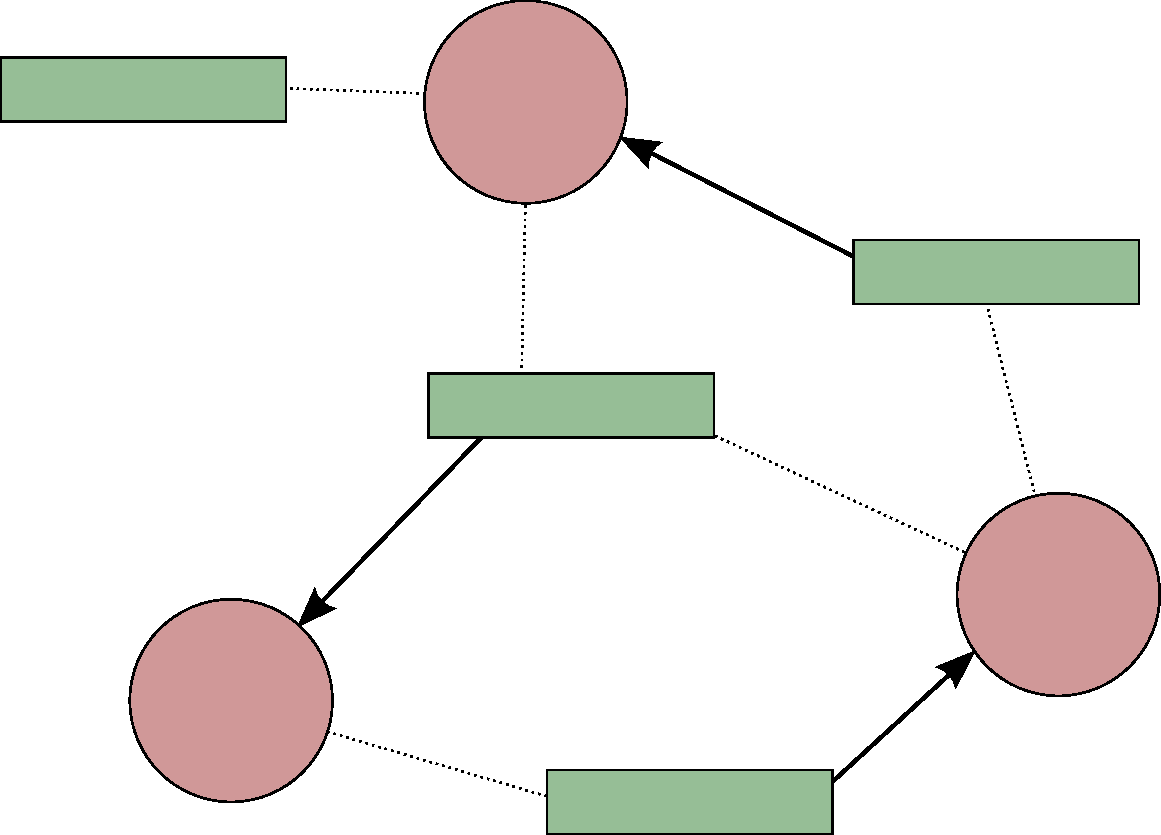
\includegraphics[width=0.8\textwidth]{img/orthograph_graph.pdf}
	\end{center}
	\caption{A two-dimensional graph. The ortholog groups (OG) are connected to the
	candidate hit transcripts by the e-value of the HMM search. Traversing the graph
	by e-value and assigning the transcripts to the OG with the best
	hit results in transcript 2 being assigned to OG A, transcript 3 to OG B and
	transcript 4 to OG C. Transcript 1 remains unassigned because the HMM search
	e-value for OG A is higher than the e-value for transcript 2.}
	\label{fig:graph}
\end{figure}

\clearpage

\addcontentsline{toc}{chapter}{Bibliography}
\bibliographystyle{plainnat}
\bibliography{/home/malty/thesis/bib/diploma}

\appendix

\chapter{Listings}
%\lstinputlisting[caption=Inserting random nucleotides at random intervals at a given probability, label=lst:randomframeshifts]{scripts/insertrandomframeshifts.pl}


\addcontentsline{toc}{chapter}{Eigenst\"andigkeitserkl\"arung}
Ich versichere hiermit an Eides statt, dass die vorliegende Diplomarbeit
selbstständig verfasst und keine weiteren als die angegebenen Hilfsmittel
benutzt sowie die Stellen der Arbeit, die in anderen Werken dem Wortlaut oder
dem Sinn nach entnommen sind, durch Angaben der Quellen sichtbar gemacht
wurden.

\vspace{4em}

\parbox[t]{0.3\textwidth}{\dotfill}

Bonn, \today

\vspace{8em}

\author

\end{document}
